Part of the current work this semester has included the selection of the sensor (Stereolabs Zed 2 Mini) and compute element (Nvidia Jetson),
as well as the identification of viable sensor mounting points on the wheelchair. This process has been detailed in the methodology.
A preliminary 34 minute driving dataset (1920x1080 @ 24 fps) has been collected around Curtin University using a GoPro Hero 4.
The experimental setup to collect this dataset can be seen in \cref{fig:gopro_dataset_collection}, including the identified
sensor mounting point.

\begin{figure}[bp]
    \centering
    \includegraphics[width=0.45\linewidth,angle=270,origin=c]{images/gopro_dataset_collection.jpg}
    \caption{Experimental setup for preliminary dataset collection}
    \label{fig:gopro_dataset_collection}
\end{figure}

The remaining technical progress this semester has focused on the evaluation of various algorithms for scene understanding
and assistive control, as well as writing the software required to evaluate these algorithms.

YOLOv5 \cite{ultralyticsYOLOv5} was one of the first algorithms evaluated for object detection.
The implementation of YOLOv5 includes an inbuilt video encoder and decoder, which simplified
the evaluation process significantly; only some preprocessing of our video dataset was required (using ffmpeg).
YOLOv5 has 5 model sizes (nano, small, medium, large, extra large),
with smaller models sacrificing accuracy for speed.
Due to the low latency requirements of a fast moving wheelchair, this algorithm was evaluated using the small model size.

YOLOv5 was evaluated on our Curtin video dataset. As seen in \cref{fig:yolov5s}, this algorithm can identify pedestrians and vehicles with high accuracy.
The confidence of the algorithm decreases when objects are further away, as can be seen with the cars in the background.
YOLOv5 ran in real-time (using a GTX 1080) on the 24 fps Curtin video dataset.

\begin{figure}[H]
    \centering
    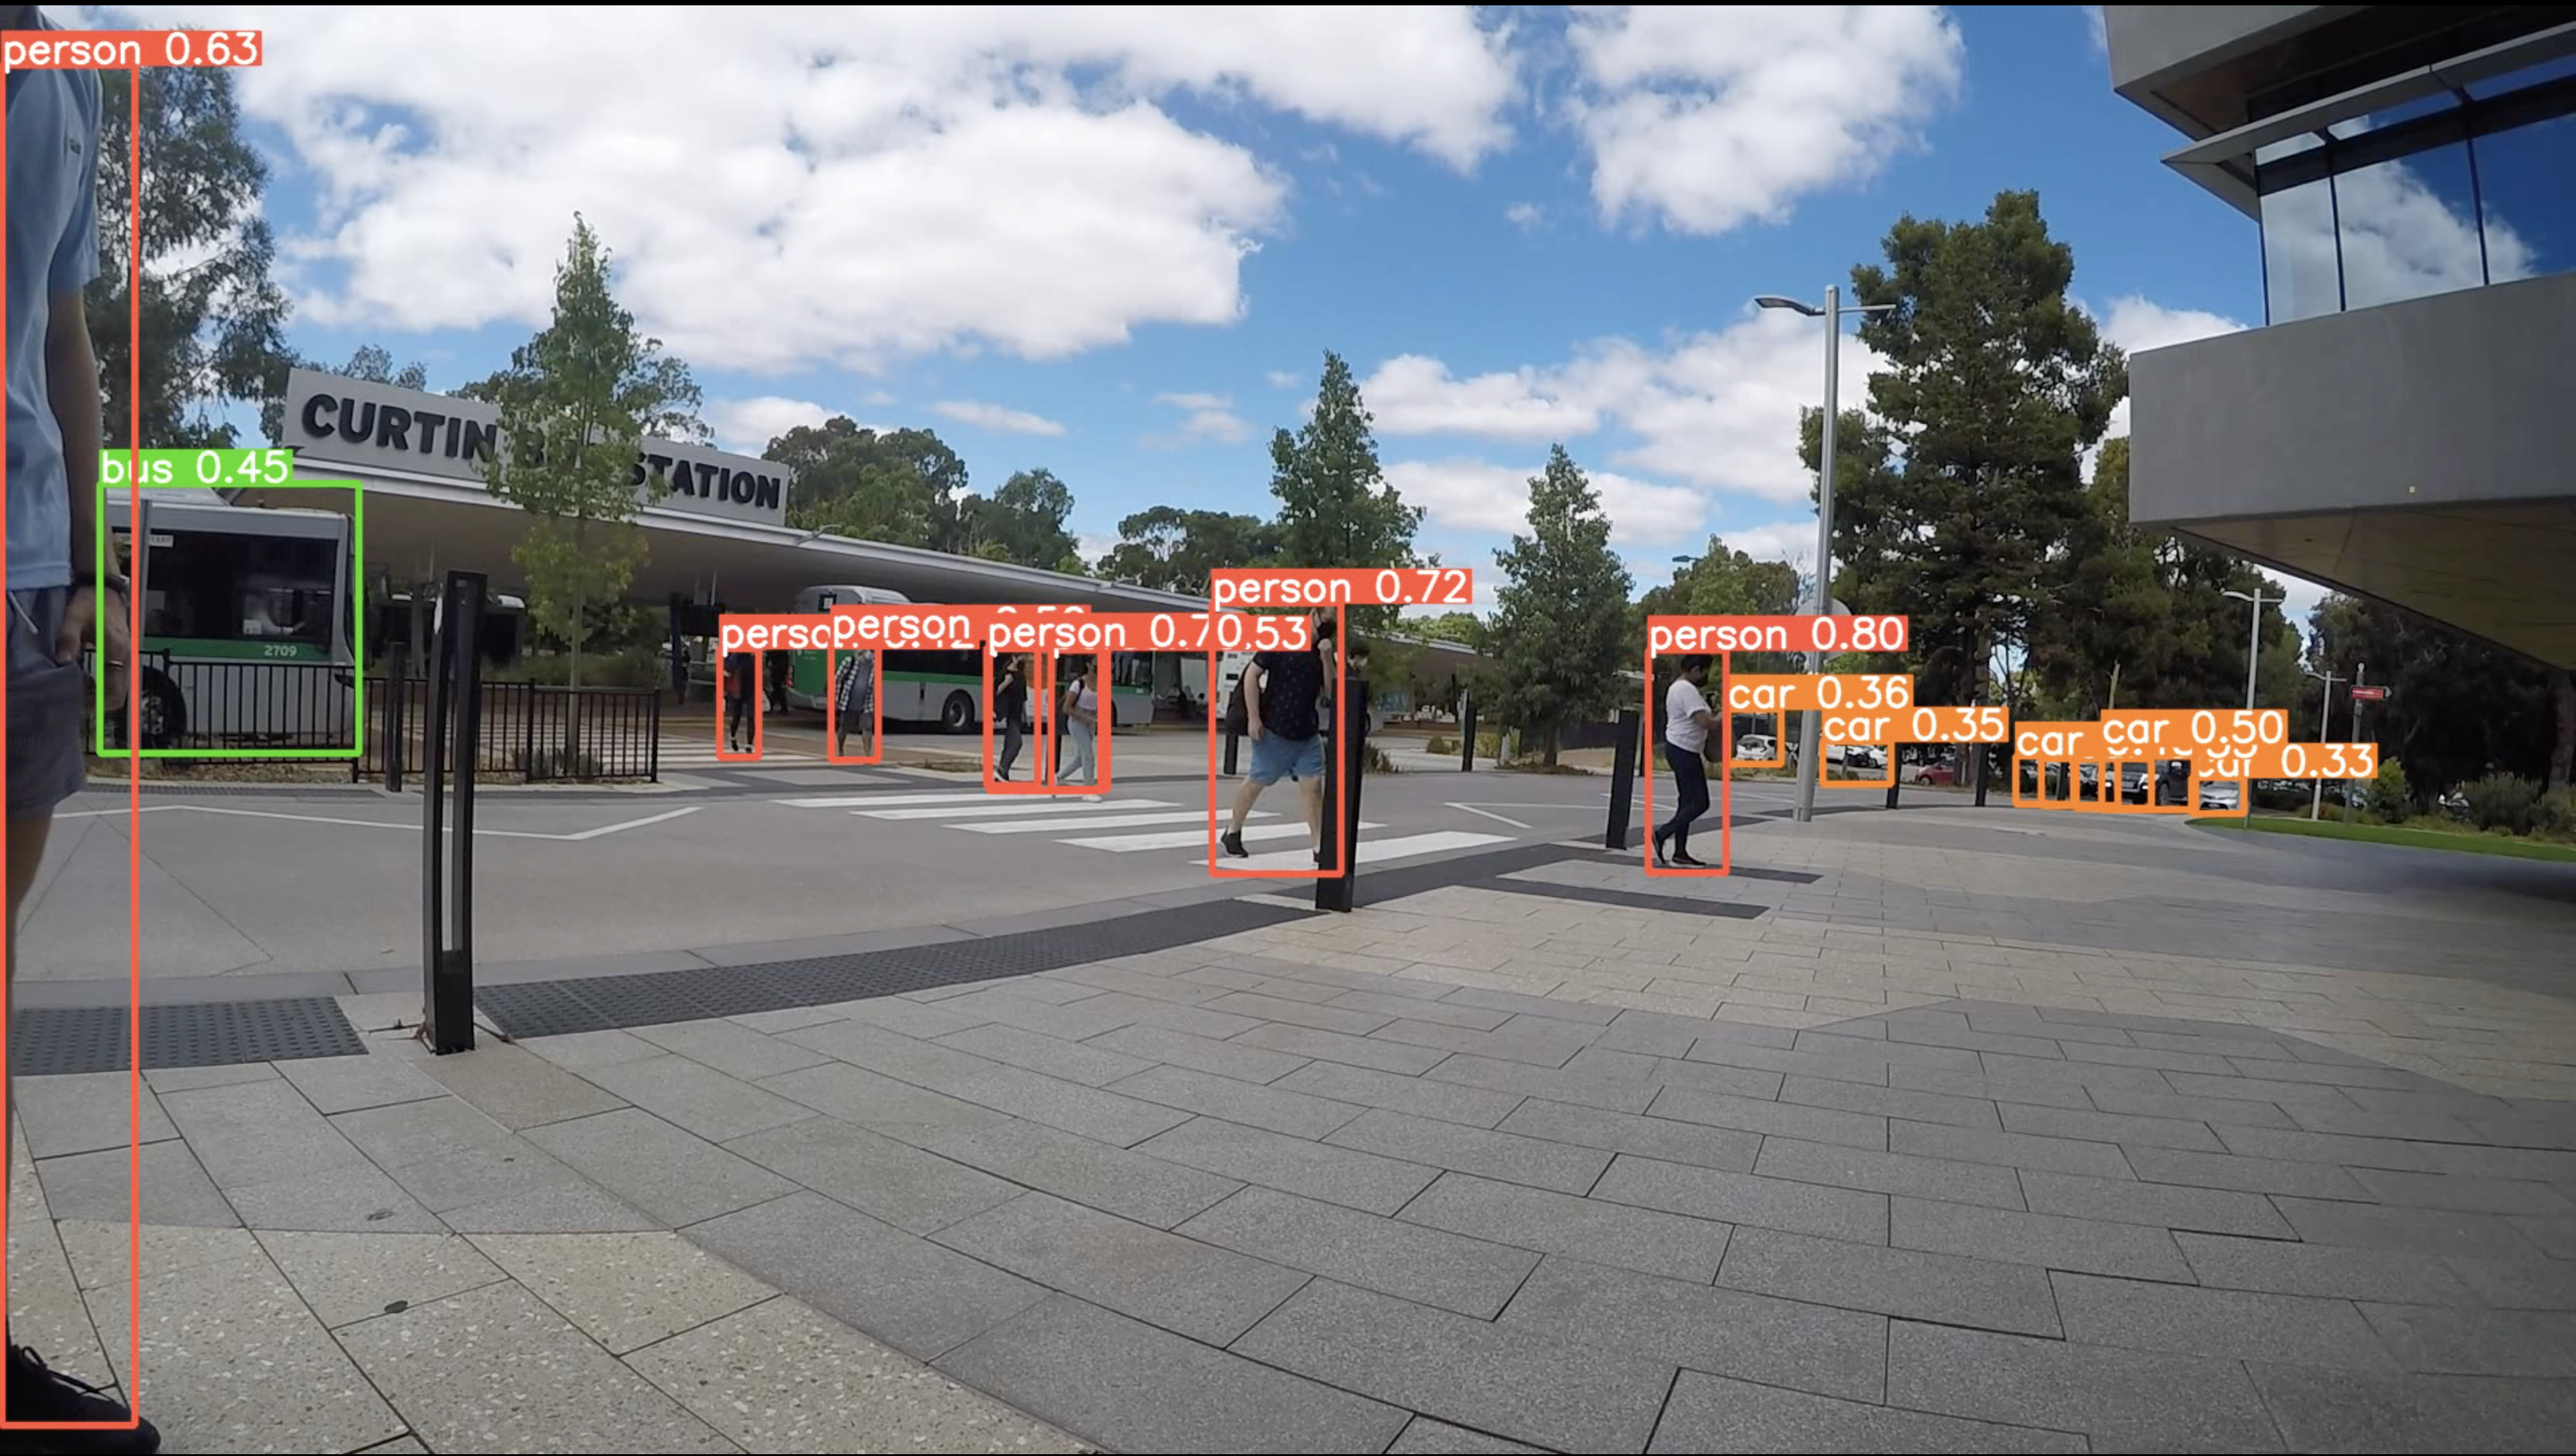
\includegraphics[width=0.65\linewidth]{images/yolov5s.png}
    \caption{YOLOv5s evaluated on the Curtin dataset}
    \label{fig:yolov5s}
\end{figure}

The next algorithm evaluated was DeepLabv3 \cite{chenRethinkingAtrousConvolution2017}. This is a segmentation algorithm
which classifies individual pixels within the image rather than drawing bounding boxes around an object.
Segmentation algorithms can be more suitable when environment features such as pathways and stairs need to be identified,
as these features do not have well-defined bounding boxes.

To evaluate this algorithm, a video encoder and decoder needed to be created. This was done using a Python generator,
so that frames in the video could simply be iterated over within a for loop and only decoded when required.
OpenCV \cite{bradskiOpenCVLibrary2000} was the underlying library used to decode each video frame into a BGR pixel array.
After evaluation of the algorithm, each processed frame was displayed on the screen and encoded into a video file using OpenCV.

Some scene processing algorithms do not run in real-time due to hardware limitations or performance issues.
When this occurs, some frames must be dropped during model evaluation to keep the scene model up to date and minimise latency.
The code used to do this is shown below. By measuring the amount of time taken to process and encode a frame, the current fps
and the number of frames to drop can be calculated.

\begin{minted}{python}
for frame in generate_frame():
    if frames_drop == 0:
        start_time = time.time()
        new_frame = process_frame(frame)
        push_frame(new_frame)
        elapsed = time.time() - start_time
        frames_drop = math.ceil(elapsed * p.fps) - 1
    else:
        frames_drop -= 1
\end{minted}

To avoid training the model from scratch, a pretrained model is loaded from PyTorch Hub using the code below.
As mentioned in the literature review, image segmentation algorithms can accept different image classifiers as a backbone.
In this case, MobileNetV3 \cite{howardSearchingMobileNetV32019} was used as a backbone due to its fast performance.
This model was trained on the MS COCO \cite{linMicrosoftCOCOCommon2014} dataset and runs at 15 fps on a GTX 1080.
% 15 fps

\begin{minted}[breaklines]{python}
seg_model = torch.hub.load('pytorch/vision:v0.10.0', 'deeplabv3_mobilenet_v3_large', pretrained=True)
\end{minted}

Pillow (a Python image library) was used to overlay the output on top of the original image;
an example of the model output can be seen in \cref{fig:deeplab}. To improve the speed of the model, input frames are
downscaled to 960x540, which causes a lower segmentation resolution.
DeepLabv3 identifies pedestrians with a high degree of accuracy, however
features such as vehicles are not accurately segmented due to their lower occurrence in the MS COCO dataset.

\begin{figure}[H]
    \centering
    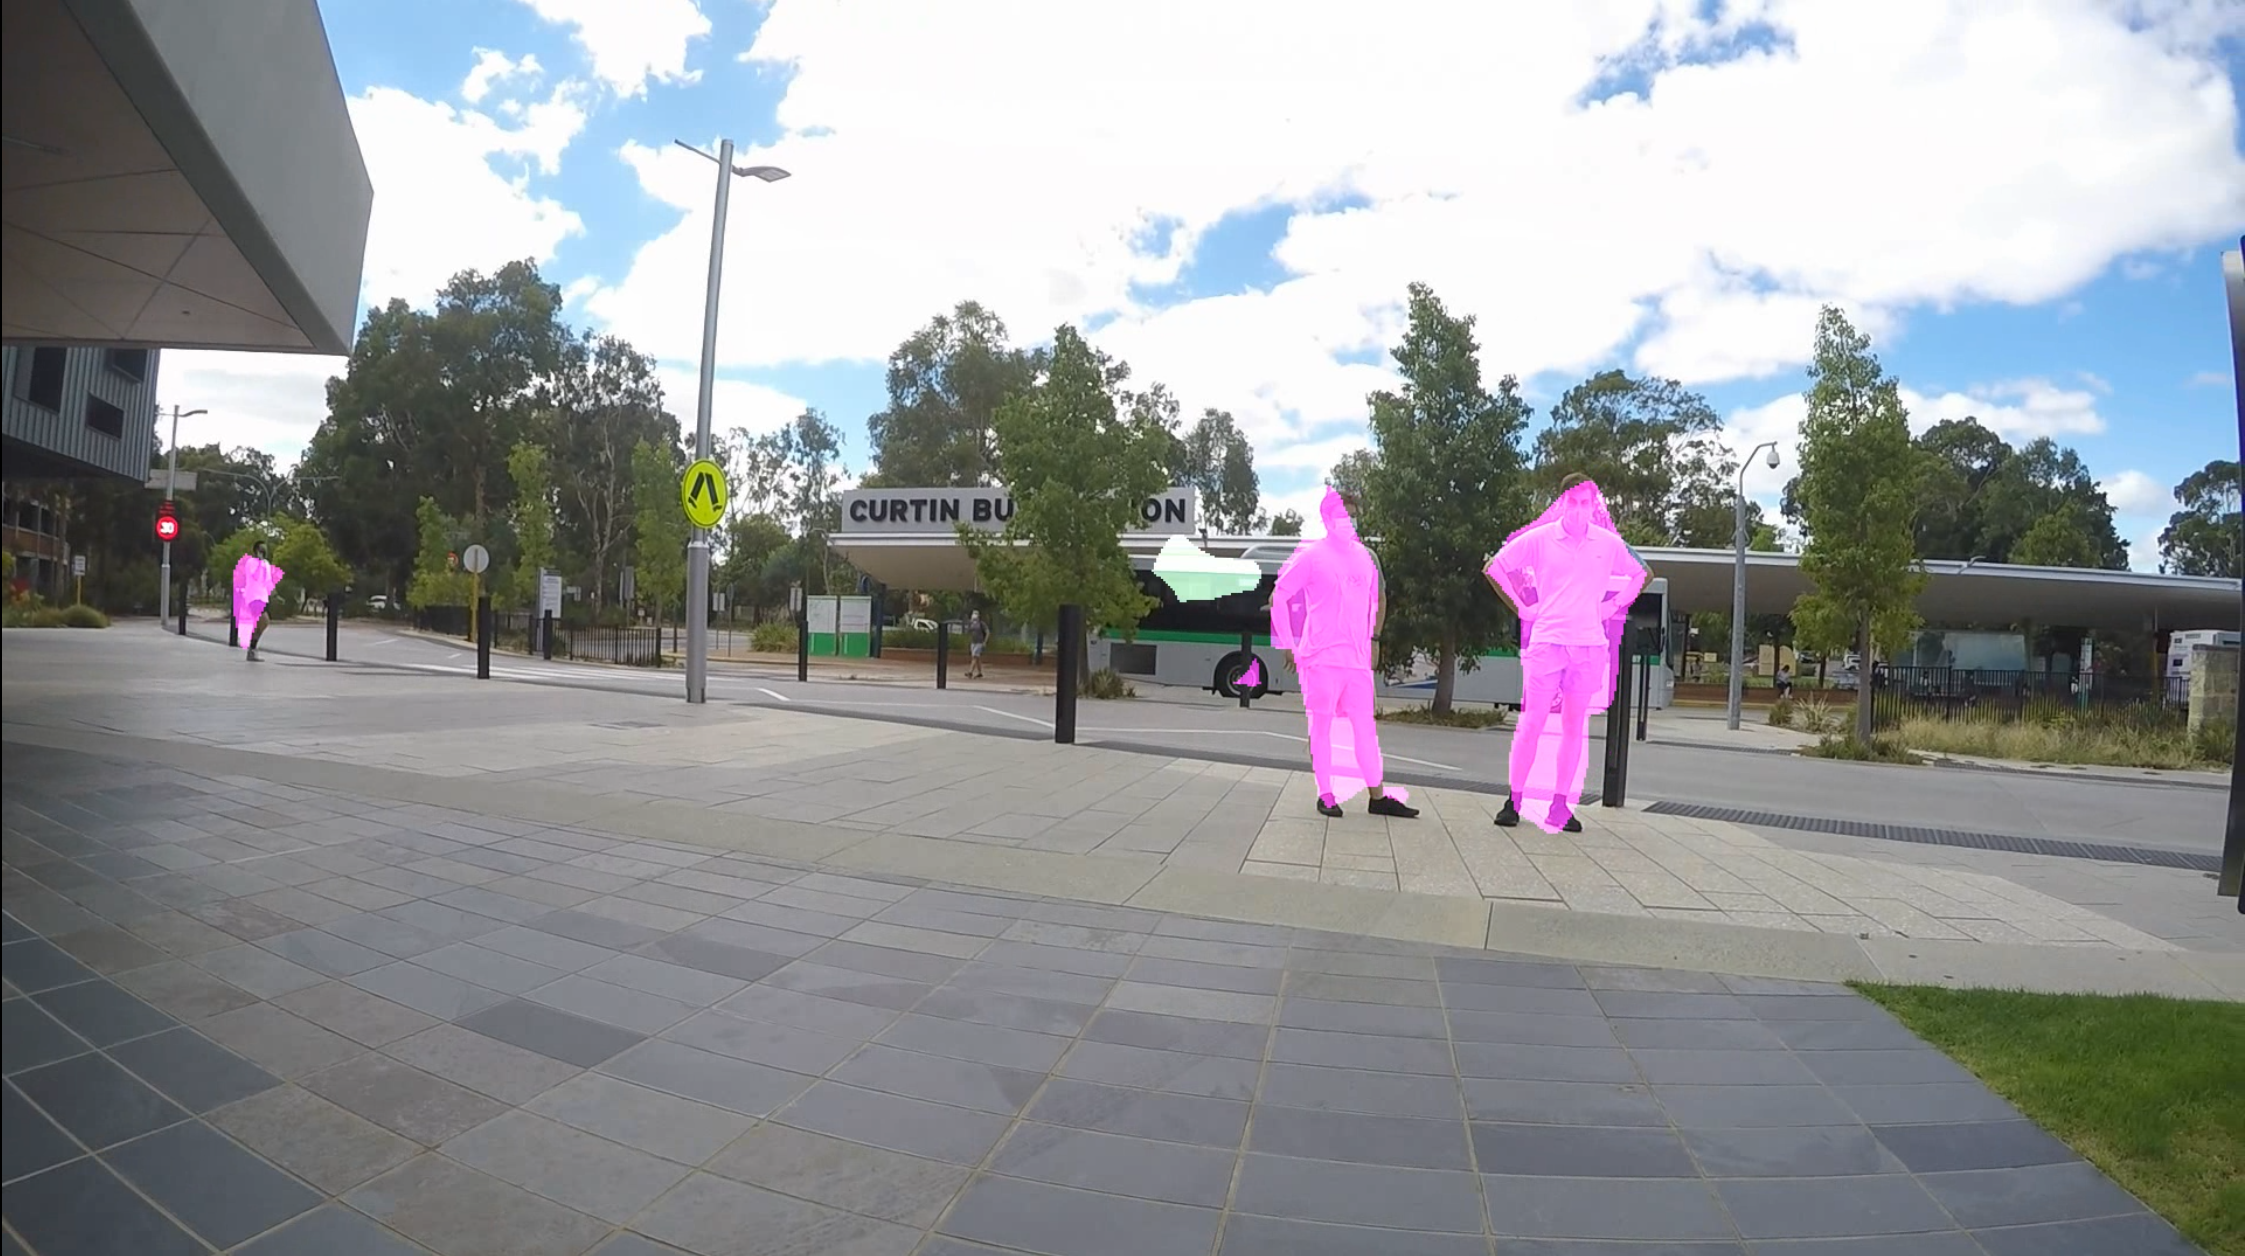
\includegraphics[width=0.65\linewidth]{images/deeplab.png}
    \caption{DeepLabv3 evaluated on the Curtin dataset}
    \label{fig:deeplab}
\end{figure}

Another model evaluated was Hybridnet \cite{vuHybridNetsEndtoEndPerception2022}, which performs drivable area segmentation
and object detection on the same backbone. In our case, drivable area segmentation was the primary focus when evaluating this model.
Code used to implement DeepLabv3 could be shared for this model, as both models were segmentation models
and loaded from PyTorch Hub. The sample code used to overlay the model output over the original image had some
performance issues, and was replaced with the code below (which was also used for our implementation of DeepLabv3).
This improved the models performance from 5 fps to 8 fps on a GTX 1080.
% 8 fps
\begin{minted}[breaklines]{python}
output = PIL.Image.fromarray(prediction)
output.putpalette(colors)
output = np.array(output.resize((width, height)).convert("RGB"))
cv2.addWeighted(frame, 1, output, 0.8, 0, frame)
\end{minted}

% perf improvement.

\Cref{fig:hybridnets_outdoor} shows Hybridnet evaluated on the Curtin dataset, with the identified drivable area highlighted.
This model performs well on uniform surfaces but has more difficulty identifying the drivable area on surfaces such as paved bricks.
This could be due to domain adaptation problems, as this model was trained on the Berkeley DeepDrive dataset \cite{yuBDD100KDiverseDriving2018}
which primarily consists of bitumen roads.

Selection of a final drivable area segmentation model is unable to be made at this stage, as further experimentation and model training
will be required. The Future Work section of this progress report details the next steps for model evaluation.
As Hybridnet also performs object detection on the same backbone, it could remove the need for a second object detection model,
which could improve the performance of the autonomous system.

\begin{figure}[H]
    \centering
    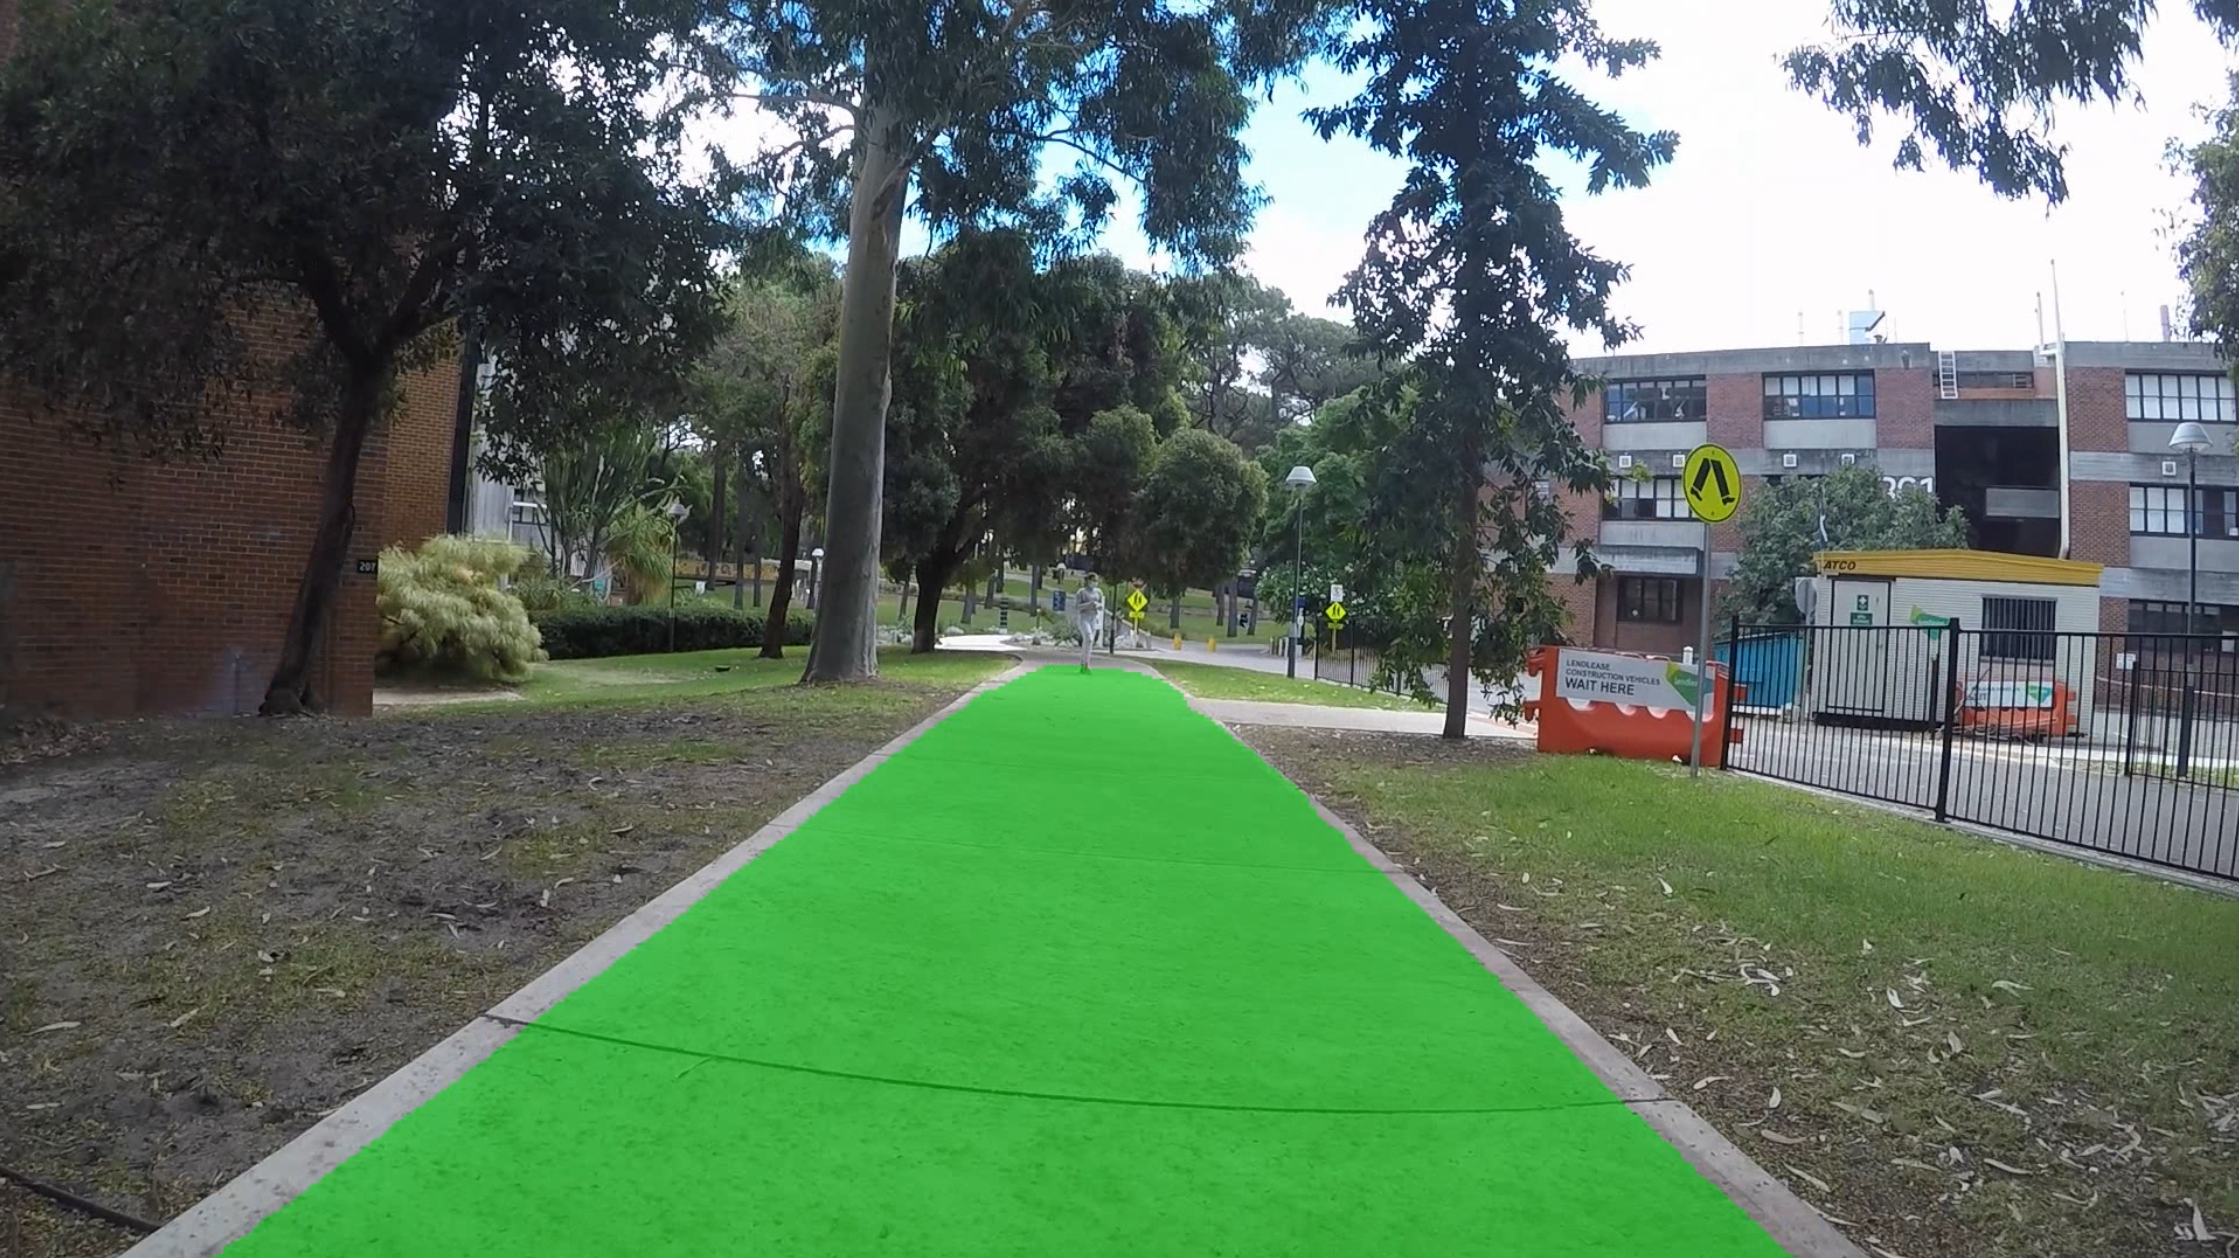
\includegraphics[width=0.6\linewidth]{images/hybridnets_outdoor.png}
    \caption{Hybridnet drivable area segmentation evaluated on the Curtin dataset}
    \label{fig:hybridnets_outdoor}
\end{figure}

Assistive control is required to navigate the wheelchair after a map of the surroundings has been built.
The VFH+ (vector field histogram) \cite{ulrichVFHReliableObstacle1998} algorithm was evaluated
in MATLAB using the Navigation toolbox and Lidar toolbox.
First, a simulated 2D environment and occupancy grid were loaded,
and a Lidar sensor was simulated at the position of the wheelchair. This code is below;
\Cref{fig:simulated_lidar} shows the occupancy grid on the left and simulated
Lidar scan on the right.

\begin{minted}[breaklines]{matlab}
load('occupancy-warehouse.mat')
show(map)
pose = [4 4 0];
helperPlotRobot(ax, pose);
lidar = rangeSensor;
[ranges, angles] = lidar(pose, map);
scan = lidarScan(ranges, angles);
plot(scan)
\end{minted}

\begin{figure}[H]
    \centering
    \includegraphics[width=0.5\linewidth]{images/simulated_lidar.png}
    \caption{Simulated occupancy grid and Lidar sensor}
    \label{fig:simulated_lidar}
\end{figure}

The VFH+ controller is configured with the wheelchair size,
turning radius, and other parameters (emitted from the code below for brevity).
The simulated Lidar scan is input into the VFH+ controller, along with
the user's desired direction, as seen below. \Cref{fig:vfh_controller} shows a visualisation
of the obstacle polar histogram, as well as the target and steering direction.

\begin{minted}[breaklines]{matlab}
vfh = controllerVFH('UseLidarScan', true);
targetDirection = -pi / 2;
steerDir = vfh(scan, targetDirection);
show(vfh)
\end{minted}

\begin{figure}[H]
    \centering
    \includegraphics[width=0.65\linewidth]{images/vfh_controller.png}
    \caption{VFH+ obstacle density and steering direction}
    \label{fig:vfh_controller}
\end{figure}

VFH+ successfully finds the nearest direction to the chosen direction which avoids obstacles.
In this case, the target direction directly right of the wheelchair is
occupied by the wall, with the chosen direction avoiding this obstacle.
One disadvantage of VFH+ is that it is not able to modify the speed of the wheelchair.
If presented with an obstacle, VFH+ will attempt to steer around the obstacle at the current velocity rather than
slowing down, which may be unsafe in some scenarios.

The current work this semester has successfully identified and evaluated several algorithms for scene recognition and assistive control.
The desired hardware for the wheelchair has been selected alongside the desired mounting points, and an initial dataset has
been collected around Curtin university.
The work done this semester enables progression towards further technical work and the end of the project.
